%%
%% This is the file `HUSTtrans.tex' designed for the undergraduate translation task at Huazhong University of Science and Technology. 
%% 
%% 
%% Copyright (C) 2019~ by Zhou Feng 冯洲 <https://github.com/zfengg>
%% 
%% Annoucement:
%% Since this work is created by Zhou Feng in 2019 to help finish the undergraduate thesis at HUST more efficiently and elegantly, it can only serve for educational and academical purpose while should never be used for commercial or profitable business.
%% ONLY for the undergratuate thesis at HUST. 
%% This work has no LPPL maintenance or any other public liscenses like MIT Liscense or General Public Liscenses(GPL). Hence the author take no responsibilites for any loss of the user using this template.
%% 
%% The Current Maintainer of this work is Zhou Feng. All the advice is welcomed by sending an e-mail to the mailbox fengzhou1113@gmail.com
%% 
%% Aiming to reach more friends, this work directly and only contains the fzHUSTtrans.tex. And I have carefully included all the settings according to the offical documents and explaination after each command line.

%% This file should compiled with XeLaTex. The edit sorftware TexStudio is recommended by zhou.

%% Btw: Be aware that my purpose is to provide a friendly latex template for myself or maybe other HUSTers, so the only thing you need to do before you start your own work is to imitate the example tex file, fzHUSTtrans.tex. Good luck!

\documentclass[11pt,a4paper]{article}
%10.5pt equals 5 hao font. 

%----------------------------------------------------------------%
%% For the layout of paper
%\usepackage[tmargin=1in,bmargin=1in,lmargin=1.25in,rmargin=1.25in]{geometry}
\usepackage[top=2.54cm, bottom=2.54cm, left=3.18cm, right=3.18cm]{geometry}
\geometry{headsep=1em,footskip=2em}
\geometry{headheight=14pt}

%----------------------------------------------------------------%
%% For Math Symbols, 载入常用的数学包, 符号包
\usepackage{amsmath}
\usepackage{amsfonts}
\usepackage{amssymb}
\usepackage{mathrsfs}

%----------------------------------------------------------------%
%% For the linespace 行间距,段间距等等
\usepackage{setspace} 
% \usepackage{indentfirst} % then the first line of each title should start with a indent.
%定义标题和段落样式
%定义1.5倍行距
\renewcommand{\baselinestretch}{1.62}
\setlength{\baselineskip}{12pt} % this is used to set the fixed value of the lineskip
\setlength\parskip{\baselineskip} % set the space between the paragraphs, set the variable \parskip \baselineskip
% parindent
\setlength{\parindent}{0pt}

%----------------------------------------------------------------%
%% For the fonts (style, color, size).字体的大小,颜色,以及定义常用的字号
 \usepackage{ctex}% If you are lazy, the CTEX suit is enough.
 % Chinese Font
 \usepackage{xeCJK}% For the Chinese through XeLaTex
 \setCJKmainfont{SimSun} % set the mainfont of Chinese as songti. (serif) for  
 \setCJKsansfont{SimSun} % sans serif font for \textsf
 \setCJKmonofont{SimSun} % monospace font for \texttt
 % \punctstyle{kaiming}   % Remove the space used by symbols like comma. Special for the mainland students like us HUSTers.
 \setCJKfamilyfont{song}{SimSun}                             %宋体 song
 \newcommand{\song}{\CJKfamily{song}}                        
 \setCJKfamilyfont{kai}{KaiTi}                        		 %楷体2312  kai
 \newcommand{\kai}{\CJKfamily{kai}}  
 \setCJKfamilyfont{hwzs}{STZhongsong}                        %华文中宋  hwzs
 \newcommand{\hwzs}{\CJKfamily{hwzs}}
 % English Font
 \usepackage{fontspec}% Then you can use the fonts installed at your device. 
 \setmainfont{Times New Roman}
 \setsansfont{Times New Roman}
 \setmonofont{Times New Roman}
 %\setsansfont{[foo.ttf]} % for the fonts at this default path.
 % Font Color 利用definecolor自己可以定义颜色
 \usepackage{xcolor}
 \definecolor{MSBlue}{rgb}{.204,.353,.541}
 \definecolor{MSLightBlue}{rgb}{.31,.506,.741}
 % Font Size (I use pinyin represents the corresponding size in Microsorft Word)
% \newcommand{\chuhao}{\fontsize{42pt}{\baselineskip}\selectfont}
% \newcommand{\xiaochuhao}{\fontsize{36pt}{\baselineskip}\selectfont}
% \newcommand{\yihao}{\fontsize{28pt}{\baselineskip}\selectfont}
% \newcommand{\erhao}{\fontsize{21pt}{\baselineskip}\selectfont}
% \newcommand{\xiaoerhao}{\fontsize{18pt}{\baselineskip}\selectfont}
% \newcommand{\sanhao}{\fontsize{15.75pt}{\baselineskip}\selectfont}
 \newcommand{\sihao}{\fontsize{14pt}{18pt}\selectfont}
 \newcommand{\xiaosihao}{\fontsize{12pt}{18pt}\selectfont}
 \newcommand{\wuhao}{\fontsize{10.5pt}{18pt}\selectfont}
% \newcommand{\xiaowuhao}{\fontsize{9pt}{\baselineskip}\selectfont}
% \newcommand{\liuhao}{\fontsize{7.875pt}{\baselineskip}\selectfont}
% \newcommand{\qihao}{\fontsize{5.25pt}{\baselineskip}\selectfont}



%----------------------------------------------------------------%
%% For the header and footer. 页眉,页脚
 \usepackage{fancyhdr} % Then you can specialize the header and footer for your own use.
 %设置页眉样式
 \newcommand{\headstyle}{
 	\fancyhead[C]{ \hwzs\wuhao 华中科技大学本科生毕业设计(论文)参考文献译文}
 }
 %设置页脚样式
 \newcommand{\footstyle}{\fancyfoot[C]{\normalfont \thepage}
 	\fancyfoot[L]{\rule[5pt]{6.7cm}{0.4pt}}
 	\fancyfoot[R]{\rule[5pt]{6.7cm}{0.4pt}}
 }
 \pagestyle{fancy}
 \fancyhf{} %清空原有样式
 \headstyle
 \footstyle
 %定义一种新的格式叫做main
 \fancypagestyle{main}{%
 	\fancyhf{} %清空原有样式
 	\headstyle
 	\footstyle
 }
% \renewcommand{\headrulewidth}{0.4pt}
% \renewcommand{\footrulewidth}{0.4pt}
% %\renewcommand{\footrule}{\rule{\textwidth}{0.4pt}}
% \lhead{} \chead{华中科技大学本科生毕业设计(论文)参考文献译文} \rhead{}
% \lfoot{} \cfoot{\thepage} \lfoot{}


 

%----------------------------------------------------------------%
%% For the styles of sections at all levels
 %设置各个标题样式
 %不需要使用part和chapter层级
 \usepackage{titlesec}
 \usepackage{titletoc}
 \titleformat{\section}{\wuhao\bfseries}{\thesection.}{1em}{} %在section标题编号后面加个点
% \titleformat*{\section}{\wuhao\bfseries} % 设置标签的形式,5号加粗
 \titleformat*{\subsection}{\wuhao\bfseries}
 \titleformat*{\subsubsection}{\wuhao\bfseries}
 % 用titlespacing修改section与正文第一行之间的距离
% \titlespacing*{\section}{0pt}{}{}
% \titlespacing*{\subsection}{0pt}{}{}
% \titlespacing*{\subsubsection}{0pt}{}{}
 \newcommand{\sectionbreak}{\clearpage} %小节从新的一页开始
%根据学校要求设置新的section, subsection, subsection, subsubsection 以及 paragraph

% For the content of section and so on
\newcommand\seccontent{
	\wuhao %默认五号字体, 行间距为1.5*\baselineskip
    \setlength{\parindent}{2em} %首段缩进两个M字符
    \setlength{\parskip}{0pt}
    }


%----------------------------------------------------------------%
%% For the style of theorems, definitions, proofs and remarks 定义数学里面一些常用的环境
\usepackage{amsthm}
\newtheorem{thm}{\textbf{定理}}[section]
 %The section in [] can be replaced by chapter or subsection
 \theoremstyle{definition} \newtheorem{law}[thm]{Law}
 \theoremstyle{plain} \newtheorem{jury}[thm]{Jury}
 \theoremstyle{remark} \newtheorem*{marg}{Margaret}


%----------------------------------------------------------------%
%% For the caption and reference 图表及公式的编号规范
\usepackage{caption}
\captionsetup[figure]{labelformat=default, labelsep=quad,name={图}}
\captionsetup[table]{labelformat=default,labelsep=quad,name={表}}
%设置图表标题的计数方式
\renewcommand{\thefigure}{\thesection--\arabic{figure}} % set caption label style to 2-1 
\renewcommand{\thetable}{\thesection--\arabic{table}} % set caption label style to 2-1 
\captionsetup[figure]{labelfont=normalfont,textfont=normalfont} 
\captionsetup[table]{labelfont=normalfont,textfont=normalfont} 
%设置图表的autoref的格式
\newcommand{\reffig}[1]{图 \ref{#1}}
\newcommand{\reftab}[1]{表 \ref{#1}}
%公式的编号格式
\numberwithin{equation}{section}
\renewcommand\theequation{\arabic{section}--\arabic{equation}}


%\DeclareCaptionFont{hust}{\normalsize}
%\captionsetup{labelsep=quad}
%\captionsetup{font={hust,singlespacing}}
%\captionsetup[figure]{position=bottom}
%\captionsetup[table]{position=top}
%\setlength{\textfloatsep}{6pt}
%\setlength{\floatsep}{0pt}
%\setlength{\intextsep}{6pt}
\setlength{\abovecaptionskip}{15pt}
%\setlength{\belowcaptionskip}{0pt}

%重新定制figure和table环境使其更好使用(这样做好处在于方便,不用再打\centering, \label之类的,但是texstudio的autoref系统无法提前预知reference的名字,觉得合适的朋友可以newenvironment.)
%\newenvironment{generalfig}[3][htbp]{
%	\def \figcaption {#2}
%	\def \figlabel {#3}
%	\begin{figure}[#1]
%		\centering
%	}{
%		\caption{\figcaption} \label{\figlabel}
%	\end{figure}
%}
%\newenvironment{generaltab}[3][htbp]{
%	\def \tabcaption {#2}
%	\def \tablabel {#3}
%	\begin{table}[#1]
%		\caption{\tabcaption} \label{\tablabel}
%		\zihao{5}
%		\centering
%	}{
%	\end{table}
%}
%% For the figures and tabulars
\usepackage{graphicx} % To include graphixs
\usepackage{booktabs} % To create three line table including the commands toprule, bottomrule, and midrule
%\usepackage{colortbl} % 

%----------------------------------------------------------------%
%% For the tableofcontents, listoftables and listoffigures, 目录 
%参考文献翻译不需要管,之后制作论文tex文档的时候需要设定
\usepackage{tocloft}
\renewcommand\contentsname{目录}
\renewcommand\listfigurename{插图目录}
\renewcommand\listtablename{表格目录} 
%\titlecontents{section} [3cm] {\bf \large}{\contentslabel{2.5em}}{}{\titlerule*[0.5pc]{$\cdot$}\contentspage\hspace*{3cm}}
%\titlecontents{标题名}[左间距]{标题格式}{标题标志}{无序号标题}{指引线与页码}[下间距]

%----------------------------------------------------------------%
%% For the bibiliograph or reference and citation
\usepackage{natbib}
\renewcommand{\refname}{\wuhao\textbf{参考文献}}
\bibsep=0pt % 用来设置每个\bibitem之间的间距
%\renewcommand{\bibname}{参考文献} % For the document class 参考文献
%\newcommand{\upcite}[1]{\textsuperscript{\textsuperscript{\cite{#1}}}} % If you want the citation label to show at the uperscript position.

%----------------------------------------------------------------%
%\usepackage{makeindex} For the index 索引
\usepackage{listings} %For the code. 代码
%----------------------------------------------------------------%
%% For the hyperlink and bookmark 超链接及书签,这样生成的pdf中的引用直接点击链接即可到达目的地
\usepackage[bookmarks=true,colorlinks,linkcolor=black,citecolor=black,urlcolor=purple]{hyperref}% 设置超链接并修改风格
%----------------------------------------------------------------%
%% For the appendix, 附录

%----------------------------------------------------------------%
% For the titlepage 标题页,此处可以省略,建议直接使用官方给出的标题页即可
\usepackage{titling} 
\title{华中科技大学本科生毕业设计 \break{(论文)参考文献翻译} \vspace{-200em}}
\author{冯洲}
\date{}

%\makeatletter % change default title style
%\renewcommand*\maketitle{%
%	\begin{center}% 居中标题
%		\normalfont % 默认粗体
%		{\sihao \@title \par} % LARGE字号
%		\vskip -1000pt% %%%  标题下面只有1em的缩进或margin
%		{\global\let\author\@empty}%
%		{\global\let\date\@empty}%
%		\thispagestyle{fancy} %  不设置页面样式
%	\end{center}%
%	\setcounter{footnote}{0}%
%}
%\makeatother

%\pretitle{\vspace{-10ex} \begin{center}\sihao} 
%  \posttitle{\par\end{center}\vspace{-8mm}}
%\preauthor{} 
%  \postauthor{} 
%\predate{} 
%	\postdate{\vspace{-400pt}}


\begin{document}
%\maketitle

\section*{\centering  {\xiaosihao 中文} {\wuhao Abc123} \\ \centering \textcolor{red}{(宋体小4号, 字母、阿拉伯数字为 Times New Romanc5号加粗, 居中)}}
\vskip -1em
\section{前言}
\seccontent \textcolor{red}{(宋体5号, 字母、阿拉伯数字为 Times New Romanc5号加粗)}

Leslie  Lamport \textbf{Leslie  Lamport}开发的\textbf{\LaTeX}是当今世界上最流行和使用最为广泛的TeX宏集。它构筑在\textbf{Plain \TeX}的基础之上,并加进了很多的功能以使得使用者可以更为方便的利用\textbf{\TeX}的强大功能。使用\textbf{\LaTeX}基本上不需要使用者自己设计命令和宏等,因为\textbf{\LaTeX}已经替你做好了。因此,即使使用者并不是很了解\textbf{\TeX},也可以在短短的时间内生成高质量的文档。对于生成复杂的数学公式,\textbf{\LaTeX}表现的更为出色\textbf{x}。\textbf{ \LaTeX}自从八十年代初问世以来,也在不断的发展.最初的正式版本为\textbf{2.09},在经过几年的发展之后,许多新的功能,机制被引入到\textbf{\LaTeX}中。在享受这些新功能带来的便利的同时,它所伴随的副作用也开始显现,这就是不兼容性。

\song
标准的\textbf{\LaTeX 2.09} 引入了“新字体选择框架”(\textbf{NFSS})的\textbf{\LaTeX、SLiTEX,AMS-\LaTeX}等等,相互之间并不兼容.这给使用者和维护者都带来很大的麻烦。为结束这种糟糕的状况,\textbf{FrankMittelbach} 等人成立了\textbf{ATeX3}项目小组,目标是建立一个最优的,有效的,统一的,标准的命令集合。即得到\textbf{\LaTeX}的一个新版本\textbf{3}.这是一个长期目标,向这个目标迈出第一步就是在\textbf{1994}年发布的\textbf{\LaTeXe}



\textcolor{red}{(宋体5号, 行间距固定1.5倍行距,字符间距为标准)}

\subsection{字体风格} \seccontent
\noindent 我是\LaTeX{}中的11pt大小的宋体. 我
{\wuhao 我是五号宋体}\textbf{3156}416 AaBc
\subsection{字体颜色} \seccontent
\textcolor{MSBlue}{微软蓝色}
\subsubsection{第三级标题}



\section{方程及图表}
$ \times\times\times\times\times\times\times\times\times\times\times\times\times\times\times\times\times\times\times\times $,其 $ \times\times\times\times\times$可表示如下:
\begin{equation}
	E_{1}=A_{1}sin\!\left(2\pi f_{1}t+\varphi_{01}+\varphi_{path1} \right)
\end{equation}
\begin{equation}
	E_{2}=A_{2}sin\!\left(2\pi f_{2}t+\varphi_{02}+\varphi_{path2} \right)
\end{equation}

$ \times\times\times\times\times\times\times\times\times\times\times\times\times\times\times\times\times\times\times\times $  (如\reftab{table1}所示)

\begin{table}[htpb]
	\centering
	\caption{样表}
	\label{table1}
	\begin{tabular}{cccc}
		\toprule
		$ \times\times\times\times\times $ & $ \times\times\times $ & $ \times\times\times $ & $ \times\times\times $ \\
		\hline
		$ \times\times\times\times\times $ & $ \times\times $       & $ \times\times $       & $ \times\times $       \\
		$ \times\times\times\times\times $ & $ \times\times $       & $ \times\times $       & $ \times\times $       \\
		$ \times\times\times\times\times $ & $ \times\times $       & $ \times\times $       & $ \times\times $       \\ 	    	\cline{2-4}
		$ \times\times\times\times\times $ & $ \times\times $       & $ \times\times $       & $ \times\times $       \\
		\bottomrule
	\end{tabular}
\end{table}
\textcolor{red}{(表标题:位于表格上方,宋体5号,字母、阿拉伯数字为Time New Roman 5号,表内容:宋体5号,字母、阿拉伯数字为Time New Roman 5号)\\ ``\fbox{\phantom{a}}''表示空格}

$ \times\times\times\times\times\times\times\times\times\times\times\times\times\times\times\times\times\times\times\times $  (如\reffig{testfig}所示)
\begin{figure}[htbp]
	\centering
	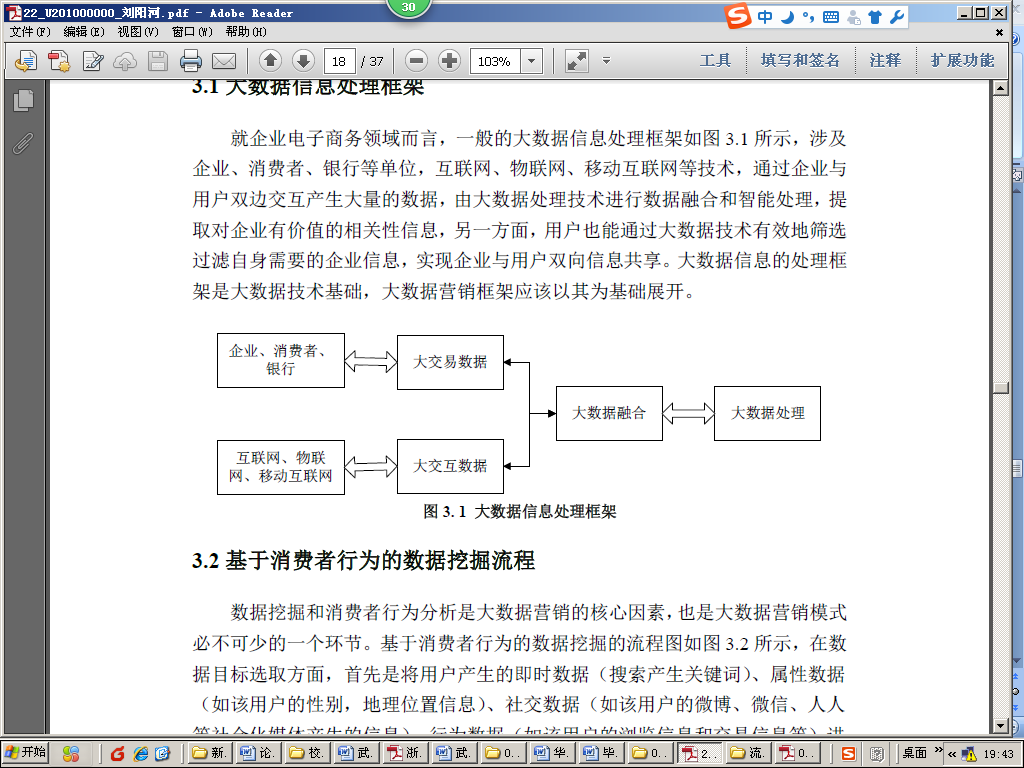
\includegraphics[width=\textwidth]{testmindmap}
	\caption{测试图片, 因为学校模板给的word中的图片就是从这上面截取的部分,所以另存为PNG之后就是这个样子}
	\label{testfig}
\end{figure}

$ \times\times\times\times\times\times\times\times\times\times\times\times\times\times\times\times\times\times\times\times $  (如\reffig{E8}所示)

\begin{figure}[htbp]
	\centering
	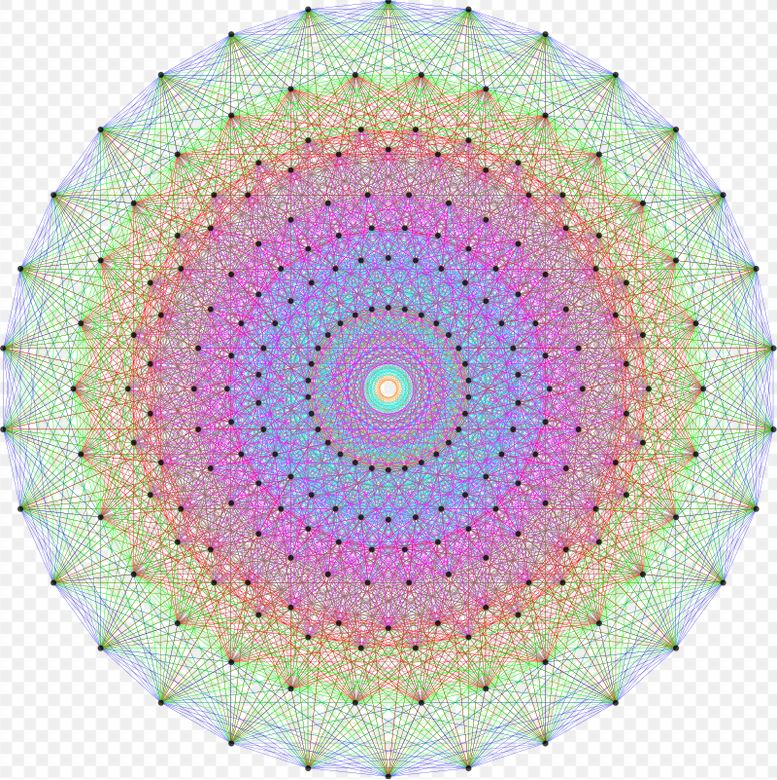
\includegraphics[width=0.5\textwidth]{E8Petrie}
	\caption{测试图片: E8 李群}
	\label{E8}
\end{figure}

\textcolor{red}{(图标题:位于图下方,宋体5号,字母、阿拉伯数字为Time New Roman 5号)}


\section{列举环境} \seccontent
\begin{description}
	\seccontent
	\item[列表]
	\item[枚举] \begin{enumerate}
			\item 图
			\item 表
		\end{enumerate}
	\item[列举] \begin{itemize}
			\item hello,world!
			\item 你好!
		\end{itemize}
\end{description}
华中科技大学本科生毕业设计(论文)参考文献译文
\sectionbreak
\section{为什么写这个tex文件}\seccontent
\subsection{背景} 每年大家都在抱怨数学公式难敲,而且敲出来不好看!确实,word的宏, 如MathType, AxMath等, 可以通过点点点来勉强解决问题,但是生成出来的公式都是一块块的,间距和大小都不好控制,更别谈交叉引用了,想起来就烦!(可能文献翻译不会有交叉引用的烦恼)。 在不考虑学习成本的情况下,\LaTeX 可以轻松搞定特别复杂的公式,而且排版特别漂亮。跟Word所见即所得(WYSIWYG: what you see is what you get)不同,\LaTeX 是所想即所得(WYWIWYG: what you want is what you get), 利用代码告诉计算机你想要什么就行了。想必大家在做文档的时候,肯定有类似的烦恼:欸? 我这里怎么忘了啥啥啥了, 那里怎么看起来有点不对劲? 这些对于\LaTeX 来说都不是问题,你只需关注内容就够了,深受科研工作者的喜爱。更何况现在基本上每个学科的主流期刊论文都是 \LaTeX 编写,而且基本都提供\LaTeX 模板。(其实很多国外大学的毕业论文都提供官方的\LaTeX 模板的,可怜的我们还要自己敲非官方的,担惊受怕的,哈哈哈!)

作为一个优秀的排版软件,\LaTeX 远不止敲公式这点儿实力,刚刚提到的方便的交叉引用,优秀的参考文献管理BiB\TeX(\url{http://www.bibtex.org/}),各种各样的格式控制,甚至可以加入编程语句来控制等等\ldots 还有,CV, 信件,学术展示(Academical Presentation, Lecture, Report...)等都可以通过\LaTeX 来变得更加优美~(反正我上次去的数学联会上的幻灯片都是\LaTeX Beamer做的,没人用PPT!) 上次用\LaTeX 写报告的体验极佳!
哎\~{}说到这儿,我更加嫌弃Word了,哈哈哈\~{}
\subsection{前期} 起初, 大概几个月前,我在网上搜现成的华科\LaTeX 参考文献翻译模板,我还真找到了一个02级学长发布在github上的套装(\url{https://hust-latex.github.io/}),然后fork到了自己的账户里面(\url{https://github.com/frenzy666/husttrans})。就在前天,我准备用的时候(我们课题组说可以拖到下学期hhh, 而且前段时间也挺忙的。),我方了。不仅它的格式要求和现在完全不一样了,而且这个模板文件搞得特别麻烦。麻烦在它给的是ins和dtx文件(理解成生成sty和cls文件的前期材料就可以啦),编译他们的时候,还要l3docstrip.tex文件(另外一个包里面用来分离ins中文本的tex文件)。好,这些都搞定之后,我得到了最终的tex文件,编译出了pdf,但是不仅缺字体,而且格式不符合要求。于是,我开始着手直接敲tex头文件,而且对前提条件的要求不能太高,要简单粗暴,要最后直接修改样本就可以使用。然后就是这个tex文件了。

后来,我也找到了一个17年的学长的研究生毕业论文cls文件(\url{https://github.com/skinaze/HUSTPaperTemp}),但是也是不好编译,容易出问题,而且cls文件的修改的语法要比tex文件麻烦,更何况这个的其他格式不符合我科论文翻译的要求。

\subsection{优缺点}
\begin{description}
	\seccontent
	\item[优点1] Tex文件简单粗暴,想要修改什么直接在头文件里面改就行了, 不需要再编译ins或者dtx之类的。而且我的注释写得还比较详细的,参数的含义也好懂。根据不同要求可以再进行改进,完全定制化。
	\item[优点2] 编译的必备条件不高,只要正确配置了TexStudio应该都可以正常编译,记得编译器选Xe\LaTeX。
	\item[优点3] 学习成本低,直接找到样本pdf相应位置修改对应的代码就可以的。
	\item[缺点] 对于第一使用\LaTeX 的朋友来说,可能花一段时间熟悉适应。tex文件头可能显得比较臃肿,第一次编译起来大概得2秒左右,后面就0.5秒吧。不过再TexStudio的快捷键的帮助下用起来挺不错的。
\end{description}


\section{使用说明}\seccontent
\begin{description}
	\seccontent
	\item[基本信息] 作者:冯洲 \href{mailto:fengzhou1113@gmail.com}{fengzhou1113@gmail.com}. 版本信息:2019/1/23, v1.0发布在 \url{https://github.com/zfengg/HUSTtex}。 如果有任何建议及纠正,欢迎邮件联系作者,非常感谢!
	\item[必备条件]  安装最新版本的 [TeXLive](\url{http://www.tug.org/texlive/})(推荐)或 [MiKTeX](\url{http://miktex.org/})。请确保所有宏包都更新至最新。由于中文支持利用的是包\textbf{XeCJK},编译器请使用 Xe\LaTeX。 编辑器推荐TeXStudio(\url{http://texstudio.sourceforge.net/}). 此文件在windows平台上测试成功,其他平台如Linux,mac没试过,哈哈哈!
	\item[章节内部及其他环境内部的格式] 请在每个环境或章节后添加 $\backslash$seccontent (5号宋体,1.5倍行距)。 例如:\begin{verbatim} 
	 \section \seccontent
	 \end{verbatim}\vskip -3em
		还有就是根据要求,正文中的数字和字母要加粗,ctrl+B即可, 也比Word手动点要好。目前没找到直接设置默认加粗的办法,有方法也请联系啦~
	\item[图表引用] 图标的编号及题注已设计符合要求,如要引用, 请使用$\backslash$reffig$\lbrace\rbrace$ 引用图,$\backslash$reftab$\lbrace\rbrace$引用表格,以达到要求样式。
	\item[公式交叉引用] 方程的编号已调好,但是引用的格式我没有另外设计,因为引用的地方可能把公式叫法不同,引用请使用自带的$\backslash$ref$\lbrace\rbrace$
	\item[距离控制] 这个tex文件的距离控制可能不太精细,如果有具体的标准数值请联系,作者来完善!
	\item[页眉页脚] 页眉页脚的样式已经调好,距页边缘的应该也没错。如果知道精确的距离请邮件通知我,我马上调整,谢谢!
	\item[超链接及书签] 利用hyperref包,每个link, cite, url已调整成超链接,点击即可到达相应位置。pdf书签及链接的样式请在头文件处根据自己的喜好修改。
	\item[参考文献] 其实论文翻译这块给的模板并没有要求参考文献,可自行删除,但是这里提供了两种参考文献的样式:第一种BiB\TeX(\url{http://www.bibtex.org/}), 第二种直接利用环境$\backslash$thebibliography.
	\item[其他] 如脚标,目录,图表目录之类的,参考文献翻译没有要求,所以我就没设计,应该不会用。如果有什么特别的需要,就直接修改头文件相应内容即可。之后我也会自己敲华科毕业论文的tex, 到时候每个细节都要改进的。
	\item[注] 这个文献翻译只包含正文部分,学校给的封面按照要求打印即可。还有参考文献原文,一般收到的是pdf,在生成pdf之后,利用Adobe Acrobat组合一下就好啦!
\end{description}

\appendix
\phantom{\cite{eXGuru1999,DonaldKnuth1984,Rudin}}
\bibliographystyle{plain}\label{bibtexref}
\bibliography{HUSTtrans}
\begin{thebibliography}{1}
	\label{latexref}
	\seccontent
	\bibitem{rudin} 王静康,张凤宝,夏淑倩等.论化工本科专业国际认证与国内认证的“实质性”.高等工程教育研究,2014,5:1-4

	\bibitem{stone} Stone J A, Howard L P. A simple technique for observing periodic nonlinearities in Michelson interferometers. Precision Engineering,1998,22(4):220-232

\end{thebibliography}
%	
\end{document}
